%%%%%%%%%%%%%%%%%%%%%%%%%%%%%%%%%%%
%This is the LaTeX ARTICLE template for RSC journals
%Copyright The Royal Society of Chemistry 2016
%%%%%%%%%%%%%%%%%%%%%%%%%%%%%%%%%%%

\documentclass[twoside,twocolumn,9pt]{article}
\usepackage{extsizes}
\usepackage[super,sort&compress,comma]{natbib} 
\usepackage[version=3]{mhchem}
\usepackage[left=1.5cm, right=1.5cm, top=1.785cm, bottom=2.0cm]{geometry}
\usepackage{balance}
\usepackage{mathptmx}
\usepackage{sectsty}
\usepackage{graphicx} 
\usepackage{lastpage}
\usepackage[format=plain,justification=justified,singlelinecheck=false,font={stretch=1.125,small,sf},labelfont=bf,labelsep=space]{caption}
\usepackage{float}
\usepackage{fancyhdr}
\usepackage{fnpos}
\usepackage[english]{babel}
\addto{\captionsenglish}{%
  \renewcommand{\refname}{Notes and references}
}
\usepackage{array}
\usepackage{droidsans}
\usepackage{charter}
\usepackage[T1]{fontenc}
\usepackage[usenames,dvipsnames]{xcolor}
\usepackage{setspace}
\usepackage[compact]{titlesec}
\usepackage{hyperref}
%%%Please don't disable any packages in the preamble, as this may cause the template to display incorrectly.%%%


\usepackage{epstopdf}%This line makes .eps figures into .pdf - please comment out if not required.

\definecolor{cream}{RGB}{222,217,201}

\begin{document}

\pagestyle{fancy}
\thispagestyle{plain}
\fancypagestyle{plain}{
%%%HEADER%%%
\renewcommand{\headrulewidth}{0pt}
}
%%%END OF HEADER%%%

%%%PAGE SETUP - Please do not change any commands within this section%%%
\makeFNbottom
\makeatletter
\renewcommand\LARGE{\@setfontsize\LARGE{15pt}{17}}
\renewcommand\Large{\@setfontsize\Large{12pt}{14}}
\renewcommand\large{\@setfontsize\large{10pt}{12}}
\renewcommand\footnotesize{\@setfontsize\footnotesize{7pt}{10}}
\makeatother

\renewcommand{\thefootnote}{\fnsymbol{footnote}}
\renewcommand\footnoterule{\vspace*{1pt}% 
\color{cream}\hrule width 3.5in height 0.4pt \color{black}\vspace*{5pt}} 
\setcounter{secnumdepth}{5}

\makeatletter 
\renewcommand\@biblabel[1]{#1}            
\renewcommand\@makefntext[1]% 
{\noindent\makebox[0pt][r]{\@thefnmark\,}#1}
\makeatother 
\renewcommand{\figurename}{\small{Fig.}~}
\sectionfont{\sffamily\Large}
\subsectionfont{\normalsize}
\subsubsectionfont{\bf}
\setstretch{1.125} %In particular, please do not alter this line.
\setlength{\skip\footins}{0.8cm}
\setlength{\footnotesep}{0.25cm}
\setlength{\jot}{10pt}
\titlespacing*{\section}{0pt}{4pt}{4pt}
\titlespacing*{\subsection}{0pt}{15pt}{1pt}
%%%END OF PAGE SETUP%%%

%%%FOOTER%%%
\fancyfoot{}
\fancyfoot[LO,RE]{\vspace{-7.1pt}
\includegraphics[height=9pt]{head_foot/LF}}
\fancyfoot[CO]{\vspace{-7.1pt}\hspace{13.2cm}
\includegraphics{head_foot/RF}}
\fancyfoot[CE]{\vspace{-7.2pt}\hspace{-14.2cm}
\includegraphics{head_foot/RF}}
\fancyfoot[RO]{\footnotesize{\sffamily{1--\pageref{LastPage} ~\textbar  \hspace{2pt}\thepage}}}
\fancyfoot[LE]{\footnotesize{\sffamily{\thepage~\textbar\hspace{3.45cm} 1--\pageref{LastPage}}}}
\fancyhead{}
\renewcommand{\headrulewidth}{0pt} 
\renewcommand{\footrulewidth}{0pt}
\setlength{\arrayrulewidth}{1pt}
\setlength{\columnsep}{6.5mm}
\setlength\bibsep{1pt}
%%%END OF FOOTER%%%

%%%FIGURE SETUP - please do not change any commands within this section%%%
\makeatletter 
\newlength{\figrulesep} 
\setlength{\figrulesep}{0.5\textfloatsep} 

\newcommand{\topfigrule}{\vspace*{-1pt}% 
\noindent{\color{cream}\rule[-\figrulesep]{\columnwidth}{1.5pt}} }

\newcommand{\botfigrule}{\vspace*{-2pt}% 
\noindent{\color{cream}\rule[\figrulesep]{\columnwidth}{1.5pt}} }

\newcommand{\dblfigrule}{\vspace*{-1pt}% 
\noindent{\color{cream}\rule[-\figrulesep]{\textwidth}{1.5pt}} }

\makeatother
%%%END OF FIGURE SETUP%%%

%%%TITLE, AUTHORS AND ABSTRACT%%%
\twocolumn[
  \begin{@twocolumnfalse}
{
\includegraphics[height=30pt]{head_foot/journal_name}\hfill\raisebox{0pt}[0pt][0pt]{
\includegraphics[height=55pt]{head_foot/RSC_LOGO_CMYK}}\\[1ex]

\includegraphics[width=18.5cm]{head_foot/header_bar}}\par
\vspace{1em}
\sffamily
\begin{tabular}{m{4.5cm} p{13.5cm} }


\includegraphics{head_foot/DOI} & \noindent\LARGE{\textbf{Ultrafast Transient Absorption Measurements of Photocarrier Dynamics in PdSe$_2$}} \\%Article title goes here instead of the text "This is the title"
\vspace{0.3cm} & \vspace{0.3cm} \\

 & \noindent\large{Guili Li,$^{}$\textit{$^{a}$} Xiaoxian Zhang,$^{}$\textit{$^{a}$} Yongsheng Wang,$^{}$\textit{$^{a}$} Zhiying Bai,$^{}$\textit{$^{a}$} Hui Zhao,$^{}$\textit{$^{b}$} Jiaqi He$^{\ast}$\textit{$^{c}$}  and Dawei He $^{\ast}$\textit{$^{a}$} } \\%Author names go here instead of "Full name", etc.

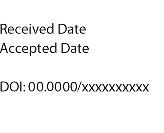
\includegraphics{head_foot/dates} & \noindent\normalsize{We investigate the photocarrier dynamics in bulk PdSe$_2$, a layered transition metal dichalcogenide with a novel pentagonal structure and unique electronic and optical properties. Using femtosecond transient absorption microscopy, we study the behavior of photocarriers in mechanically exfoliated bulk PdSe$_2$ flakes at room temperature. By employing a 400 nm ultrafast laser pulse, electron-hole pairs are generated, and their dynamics are probed using an 800 nm detection pulse. Our findings reveal that the lifetime of photocarriers in bulk PdSe$_2$ is approximately 210 ps. Furthermore, by spatially resolving the differential reflection signal, we determine a photocarrier diffusion coefficient of about 7.3 cm$^{2}$ s$^{-1}$. Based on these results, we estimate a diffusion length of around 400 nm and a photocarrier mobility of approximately 300 cm$^{2}$ V$^{-1}$ s$^{-1}$. These results shed light on the ultrafast optoelectronic properties of PdSe$_2$, offer valuable insights into photocarriers in this emerging material, and enable design of high-performance optoelectronic devices based on PdSe$_2$. } \\%The abstrast goes here instead of the text "The abstract should be..."

\end{tabular}

 \end{@twocolumnfalse} \vspace{0.6cm}

  ]
%%%END OF TITLE, AUTHORS AND ABSTRACT%%%

%%%FONT SETUP - please do not change any commands within this section
\renewcommand*\rmdefault{bch}\normalfont\upshape
\rmfamily
\section*{}
\vspace{-1cm}


%%%FOOTNOTES%%%

\footnotetext{\textit{$^{a}$~Key Laboratory of Luminescence and Optical Information, Ministry of Education,
Institute of Optoelectronic Technology, Beijing Jiaotong University, Beijing 100044,
China. E-mail: dwhe@bjtu.edu.cn}}
\footnotetext{\textit{$^{b}$~Department of Physics and Astronomy, The University of Kansas, Lawrence, Kansas
66045, USA. E-mail: huizhao@ku.edu; Fax: +1 785 864 5262; Tel: +1 785 864 1938}}
\footnotetext{\textit{$^{c}$~College of Mathematics and Physics, Beijing University of Chemical Technology, Beijing 100029, China. E-mail: jqhe@buct.edu.cn }}

%Please use \dag to cite the ESI in the main text of the article.
%If you article does not have ESI please remove the the \dag symbol from the title and the footnotetext below.



%%%END OF FOOTNOTES%%%

%%%MAIN TEXT%%%%


\section{Introduction}
The successful preparation of graphene has sparked significant interest in two-dimensional layered materials with unique optical, electrical, chemical, and thermal properties. In particular, layered transition metal dichalcogenides (TMDCs) have garnered extensive attention from researchers over the past decade due to their excellent charge transport and thermoelectric properties, layer-dependent electronic band structures, and good air stability.\cite{jariwala2017van,novoselov20162d,pan2014construction} MoS$_2$, in particular, with a moderate carrier mobility and a sizable band gap, has been widely studied.\cite{radisavljevic2011single,liu2019high} The successful fabrication of field-effect transistors (FETs) based on monolayer MoS$_2$ was reported in 2011.\cite{coleman2011two,mak2010atomically} However, its relatively large band gap (1.2-1.9 eV) \cite{manzeli20172d} and the narrow tunable band gap range hinders its optimal use in optoelectronic devices. Black phosphorus, which has also been extensively studied, offers a widely tunable band gap (0.3-2 eV); however, its air instability poses a significant challenge for practice devices.\cite{ong2014anisotropic,tran2014layer} Similarly, the more recently investigated Bi$_2$O$_2$Se system exhibits a narrow band gap (approximately 0.8 eV), limiting its application in visible optoelectronics.\cite{wu2017controlled,wu2017high}

In contrast to most TMDCs, PdSe$_2$ offer wide tunability of its physical properties by its thickness. For example, it band gap changes from 1.43 eV in a monolayer to 0.6 eV in bulk.\cite{sun2015electronic} With small band gaps, it can be used to manufacture near-infrared photodetectors, sensors, and other devices with high sensitivity and high stability. Additionally, PdSe$_2$ exhibits high carrier mobility,\cite{gu2020two}  in-plane optical anisotropy,\cite{oyedele2017pdse2} and remarkable air stability.\cite{hoffman2019exploring} FETs with PdSe$_2$ as the channel material have been demonstrate, with high charge mobilities and superior bipolar characteristics.\cite{qin2018monolayer}  Theoretical calculations have predicted that the carrier mobility of pentagonal two-dimensional PdSe$_2$ can exceed 1000 cm$^{2}$/Vs, while experimentally achieved values are below 300 cm$^{2}$/Vs.\cite{gu2020two,sun2015electronic,chow2017high,Di2020Electron} While such a mobility is moderate compared to other narrow-gap 2D materials, the high stability of PdSe$_2$ in air enhances the operational lifetime of devices in complex environments. Furthermore, PdSe$_2$-based photodetectors demonstrate excellent performance, such as ultra-wideband spectral detection, ultrafast response and high sensitivity.\cite{long2019palladium,lu2020layer,2020High} For instance, PdSe$_2$ photodetectors have achieved a responsivity of 708 A W$^{-1}$ and a detectivity of 1.31×10$^{9}$ Jones.\cite{2019High}

In additional to these applications as individual material, PdSe$_2$ has also been used to fabricate heterostructures for photodetectors with exceptional performance. A PdSe$_2$/MoS$_2$ van der Waals heterostructure photodetector demonstrated a detectivity as high as 8.21×10$^{9}$ Jones, with excellent photocurrent response time.\cite{long2019palladium} Likewise, a PdSe$_2$/WS$_2$ heterostructure device exhibits a broadband spectral light response from 532 to 1550 nm, with a response time of less than 100 ms.\cite{kang2021van} However, despite the early study of PdSe$_2$ dating back to 1957,\cite{gronvold1957crystal} the dynamic properties of photocarrier in PdSe$_2$ have not been fully explored. These properties are crucial for the future design and optimization of FET and photodetectors based on PdSe$_2$ and its heterostructures.

In this study, we investigate the dynamics of photocarriers in mechanically exfoliated thick flakes of PdSe$_2$ using time-resolved and spatially-resolved transient absorption microscopy. We determine a lifetime of photocarriers in bulk PdSe$_2$ of approximately 210 ps, a diffusion coefficient is approximately 7.3 cm$^{2}$ s$^{-1}$, and a diffusion length of around 400 nm. The carrier lifetime is a critical factor that significantly impacts the performance of optoelectronic devices. For instance, in solar cells, the photocarrier
lifetime determines the power conversion efficiency. The diffusion length of the photocarriers has a significant impact on the performance of semiconductor optoelectronic devices, such as photodiodes and solar cells. In these devices, the diffusion length of the photocarriers determines the distance the photocarriers can reach during their lifetime, and thus impacts the detectivity and efficiency of these devices. The findings presented in this study offer valuable insights into the comprehension, design, development, and optimization of high-performance optoelectronic devices based on PdSe$_2$. Investigations of the ultrafast photocarrier dynamics also provide insights into the underlying physical mechanisms and enable the development of new device architectures and applications with improved performance.



\section{Experimental Section}
In this study, we utilized high-purity crystals of PdSe$_2$ obtained from 2D Semiconductor. The bulk PdSe$_2$ sample was prepared by mechanically exfoliating flakes from a crystal onto a polydimethylsiloxane (PDMS) substrate using an adhensive tape. Subsequently, a dry transfer technique was employed to transfer the exfoliated PdSe$_2$ flakes onto a SiO$_2$/Si substrate. During the optical microscopic examination, it was observed that thicker flakes exhibit higher contrasts. Therefore, by comparing the microscopic images, we were able to select the flakes of appropriate thickness for our experiments. We chose samples that exhibited relatively high contrasts so that they can be treated as bulk crystals. 

The photocarrier dynamics in PdSe$_2$ is studied by using a home-built transient absorption microscopy setup with space-time resolution capabilities, as illustrated in Fig. 1. An 80-MHz femtosecond titanium sapphire oscillator (MAI TAI HP by Newport) outputs ultrashort pulses with a temporal width of less than 100 fs and a wavelength range of 690-1040 nm. For our experimental requirements, the MAI TAI was adjusted to output 800-nm pulses.

The 800-nm pulse is divided into two parts through a beam splitter. One part is used as the probe pulse for the measurement, while the other part is used to generate a pump pulse of 400 nm, by passing it through a ${\beta}- $barium borate (BBO) crystal. The pump pulse is directed to the sample for photoexcitation of the carriers. The probe pulse is subsequently delivered to the sample after a delay produced by a motorized translation stage. The two pulses are spatially overlapped. When the optical path lengths of the probe and pump are equal, the two pulses arrive at the sample simultaneously, which is defined as zero delay (${\Delta} t = 0$ ). During the experiment, half-wave plates (HWPs) are used to adjust the power of the pump and probe pulses, and polarizers (PZs) are used to adjust their polarization state. A photodetector is used to detect the power of the probe pulse that is reflected off the sample, converting it to an electrical signal. A lock-in amplifier is utilized to collect and record the signal on a computer. To achieve a higher signal-to-noise ratio with the lock-in amplifier, a chopper is used to modulate the pump pulse. With this configuration, the lock-in amplifier measured the change of the detected probe power induced by the pump. This signal is proportional to the differential reflectance, $ {\Delta} R⁄R_0= (R-R_0 )/R_0$, where $R$ and $R_0$ are the probe reflectance with and without the pump pulse, respectively.

Building upon this time-resolved system, the introduction of spatially-resolved pump-probe allowed us to investigate the in-plane transport characteristics of photocarriers. By combining ultrafast time and space resolution, we were able to study the dynamics of bulk PdSe$_2$ carriers on the ultrafast timescale and µm length scales. In such measurements, the differential reflection signal was recorded as a function of the spatial distance between the centers of the probe and pump spots. By carefully adjusting the pitch angle of the reflected probe light through controlled tilting of a beam splitter in the probe optical path, the probe light was deviated from normal, enabling continuous variation of the relative position of the two spots and thus measurement of the differential reflection signal as a function of the probe delay and the probe position. Throughout the measurements, the sample was maintained at room temperature under ambient conditions.

\begin{figure}[h]
\centering
  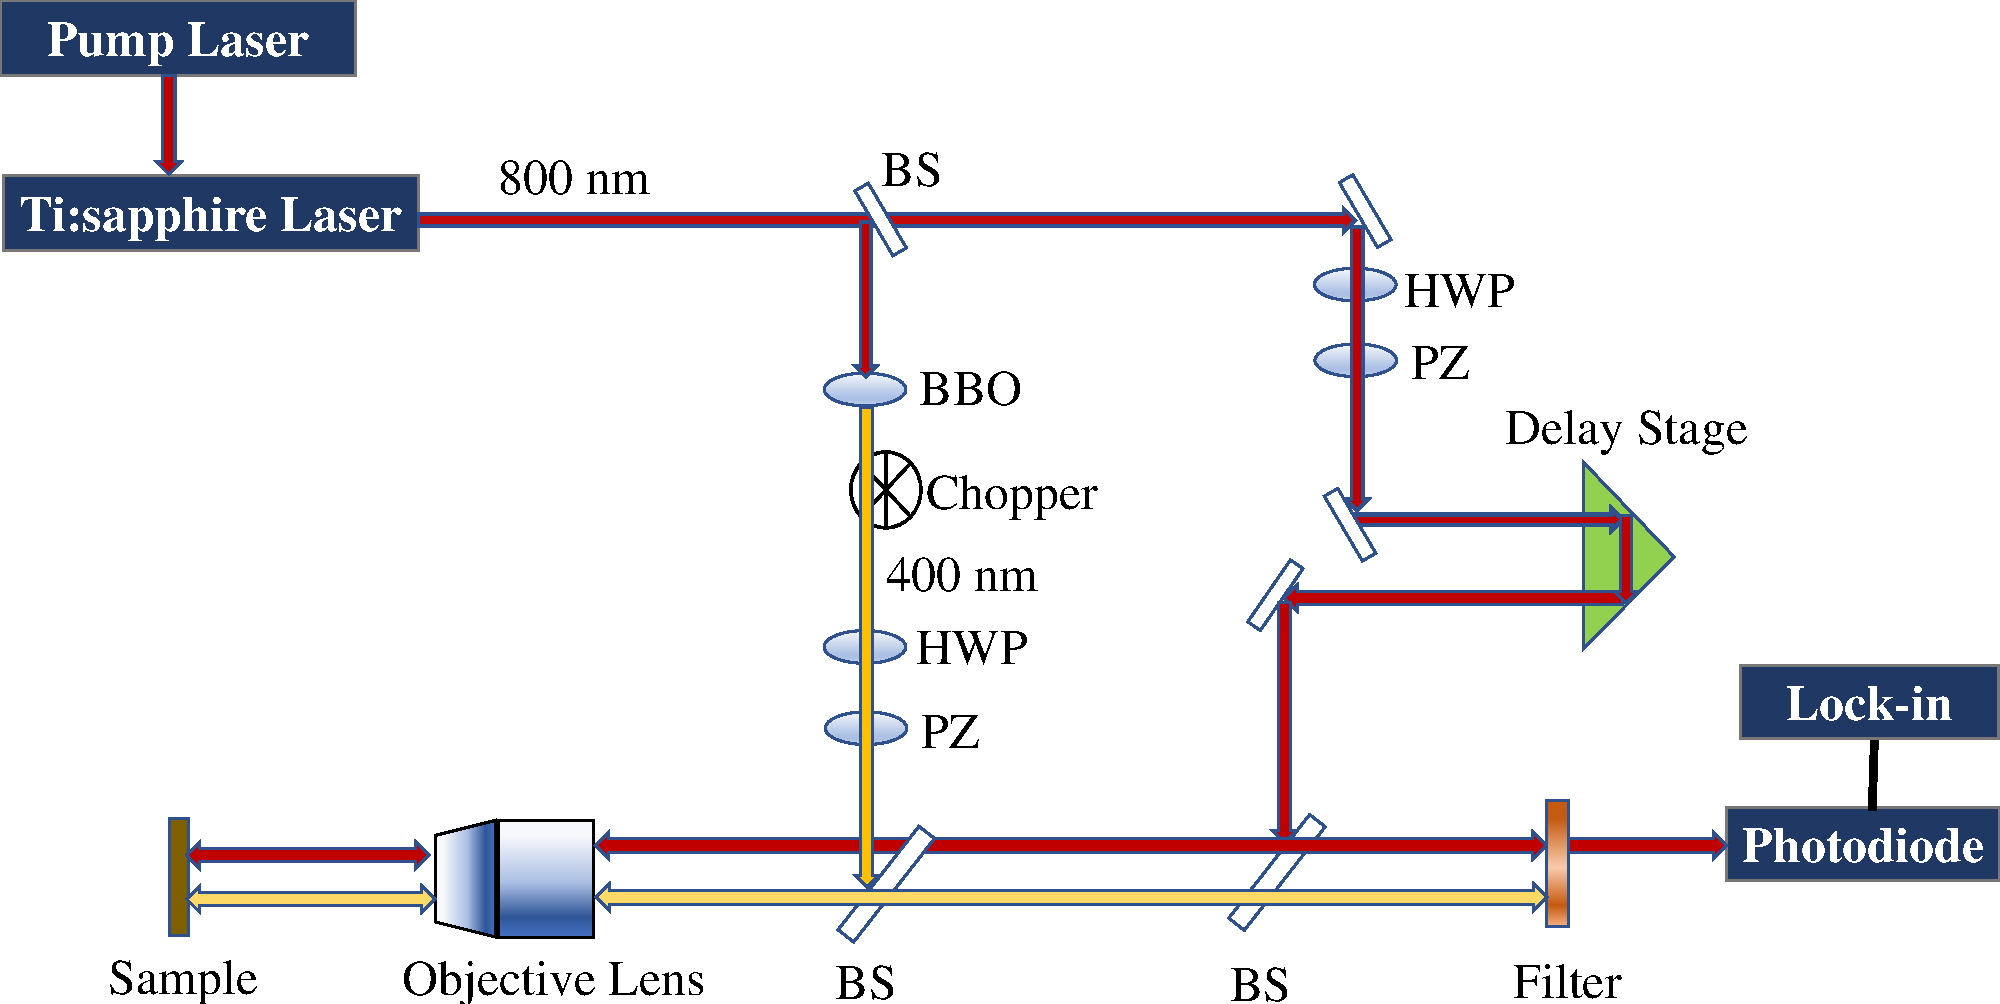
\includegraphics[height=4.5cm]{example1}
\caption{Schematics of the transient absorption microscopy setup.}
  \label{fgr:example}
\end{figure}

\begin{figure*}[h]
\centering
  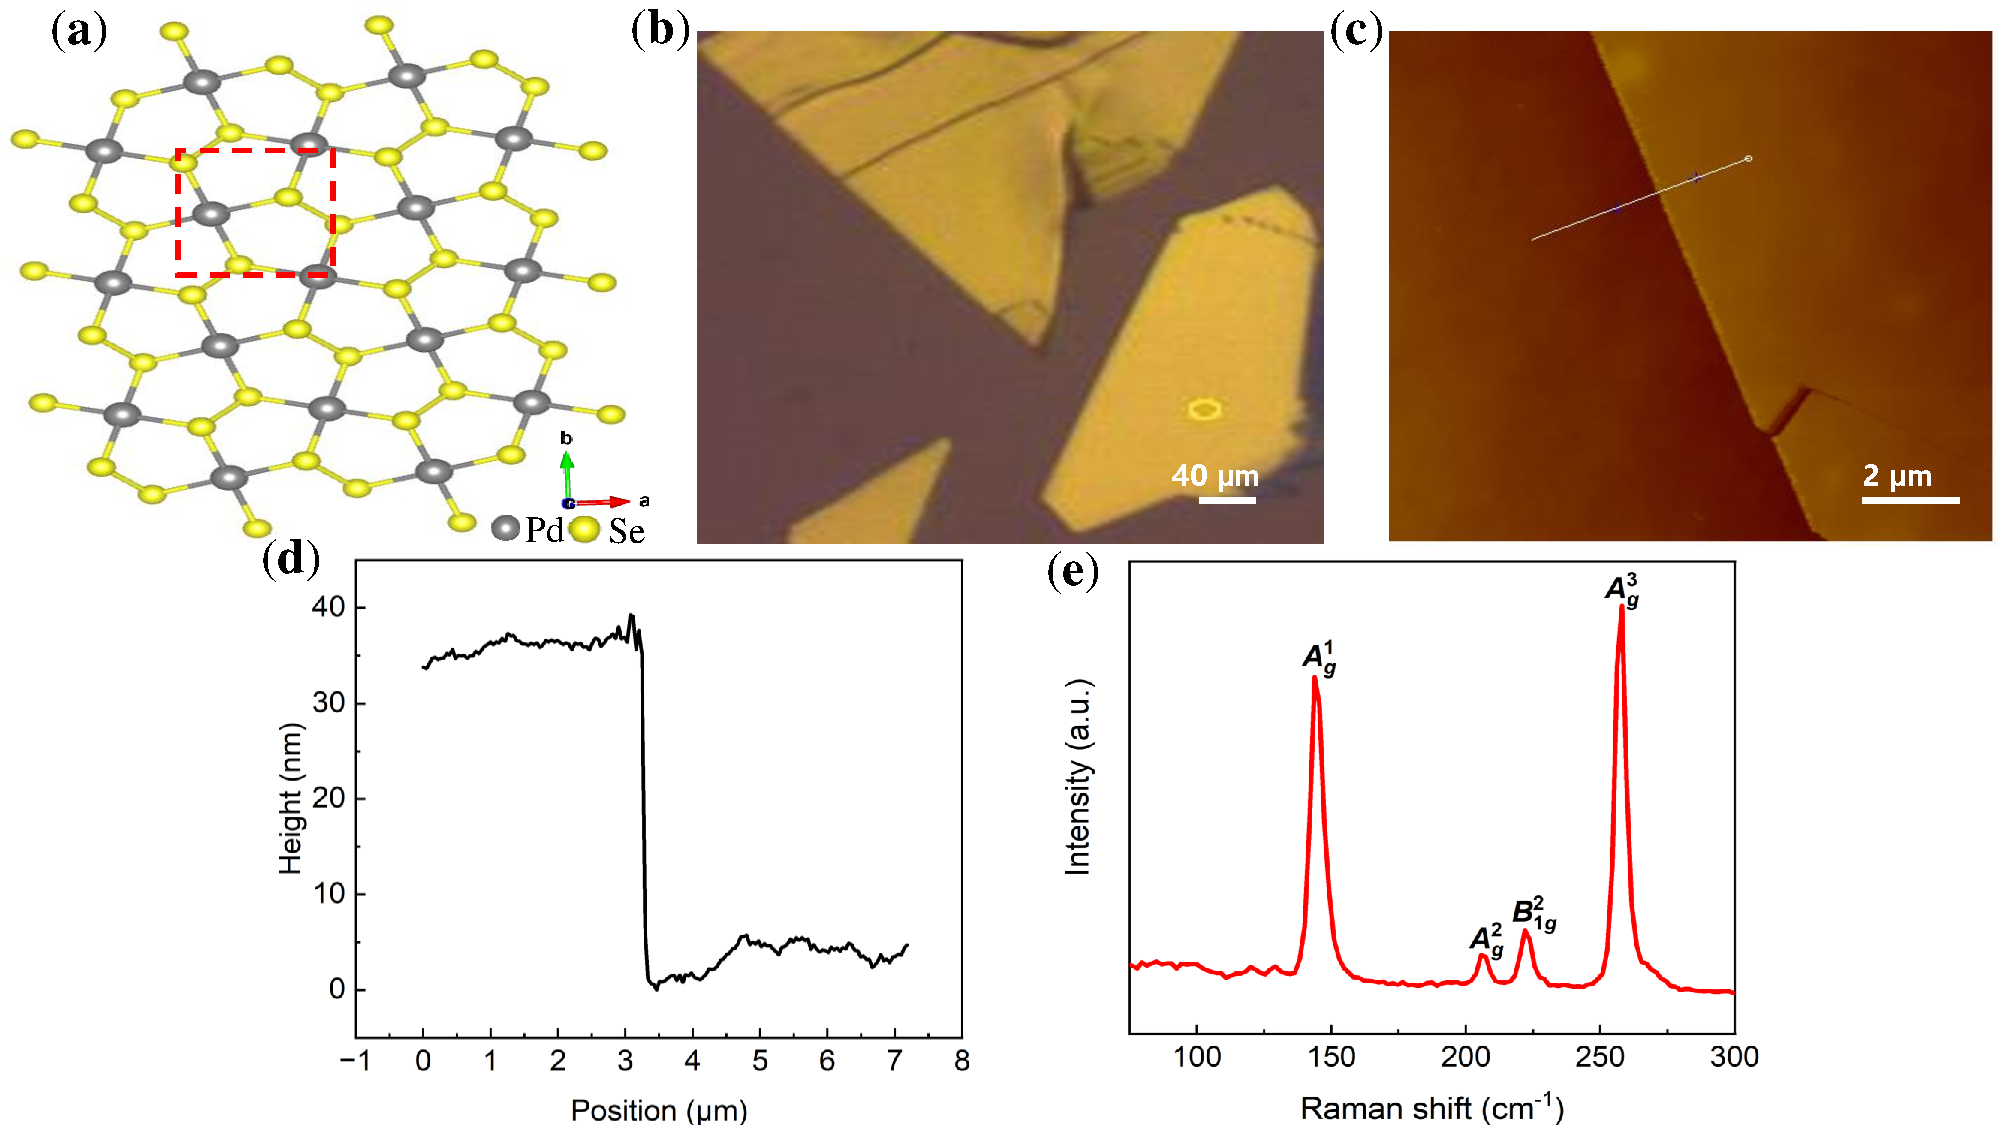
\includegraphics[height=9.6cm]{example2}
  \caption{(a) Crystalline structure of PdSe$_2$. The gray and yellow spheres represent Pd and Se atoms, respectively. (b) Optical microscope image of the bulk PdSe$_2$ sample on a SiO$_2$/Si substrate. (c) Atomic force microscope image of the PdSe$_2$ sample. (d) Height profile of the sample along the white line shown in panel c, indicating a sample thickness of approximately 33 nm. (e) Raman spectrum of the PdSe$_2$ sample shown in (b) measured with a 532 nm laser beam.}
  \label{fgr:example}
\end{figure*}

\section{Results and Discussion}
Unlike the 1T, 2H, and 1T' structures commonly found in most 2D TMDCs,\cite{chhowalla2013chemistry,kolobov2016two} PdSe$_2$ has a folded pentagonal atomic structure with an orthogonal lattice arrangement,\cite{soulard2004experimental} as shown in Fig. 2a. In this structure, each Pd atom forms covalent bonds with four Se atoms, and the Se atoms within a single layer are bonded to each other.\cite{jakhar2020pressure} The layers are connected through van der Waals forces, making the structure highly stable.

The optical microscope image of the bulk PdSe$_2$ sample in Fig. 2b reveals that the sample has an irregular shape with approximate dimensions of 86 × 200 µm$^{2}$. To further characterize the sample, a cross-sectional view by atomic force microscopy (AFM) is shown in Fig. 2c, revealing a thickness of approximately 33 nm in Fig. 2d. From the perspectives of electronic properties, the sample can be viewed as a bulk crystal as its electronic band structure is expected to be bulk-like. 



The Raman spectrum of the PdSe$_2$ sample is obtained at room temperature using a 532 nm laser, as depicted in Fig. 2e. The spectrum exhibits four distinct Raman characteristic peaks located at approximately 144 cm$^{-1}$, 206 cm$^{-1}$, 222 cm$^{-1}$, and 257 cm$^{-1}$. These peaks are in good agreement with those reported in literature for PdSe$_2$ .\cite{oyedele2017pdse2,huo2021thickness} The observed peaks are sharp, indicating the high quality of the sample. Specifically, the four peaks correspond to the $A_g^1$, $A_g^2$, $B_{1g}^2$  and $A_g^3$ vibrational modes, respectively. The $A_g^1$, $A_g^2$ and $B_{1g}^2$ modes primarily arise from the motion of the Se atoms, whereas the $A_g^3$ mode (located at approximately 257 cm$^{-1}$) is associated with the relative motion between Pd and Se atoms.



Next, we performed transient absorption measurements using an 800-nm probe and a 400-nm pump to obtain the time-resolved differential reflection signal of the sample at different pump fluences. A combined experimental and computational study shew that bulk-like PdSe$_2$ has an indirect band gap of about 0.6 eV and a direct band gap of about 1.0 eV at its ${\Gamma}$ point.\cite{wei2022layer}  Hence, the 400-nm (3.10-eV) pump excites photocarriers with large excess energies. The 800-nm (1.55-eV) probe coupled to the direct transitions in the high energy states in the ${\Gamma}$ valley, and thus monitors carrier density in these states. However, since the carrier system form a thermal distribution, these carriers represents the overall carrier population and its dynamics. Fig. 3a and 3b show examples of the observed differential reflection signals in the short (a) and long time ranges (b), respectively. It has been reported that the absorption coefficient of PdSe$_2$ at 400 nm is 5×10$^{8}$ m$^{-1}$.\cite{ye2021layer} Using this value, the areal carrier density injected by a fluence of 1 µJ cm$^{-2}$ at the center of the pump spot and at the front surface of the sample is approximately 2 × 10$^{12}$ cm$^{-2}$.

\begin{figure}[h]
\centering
  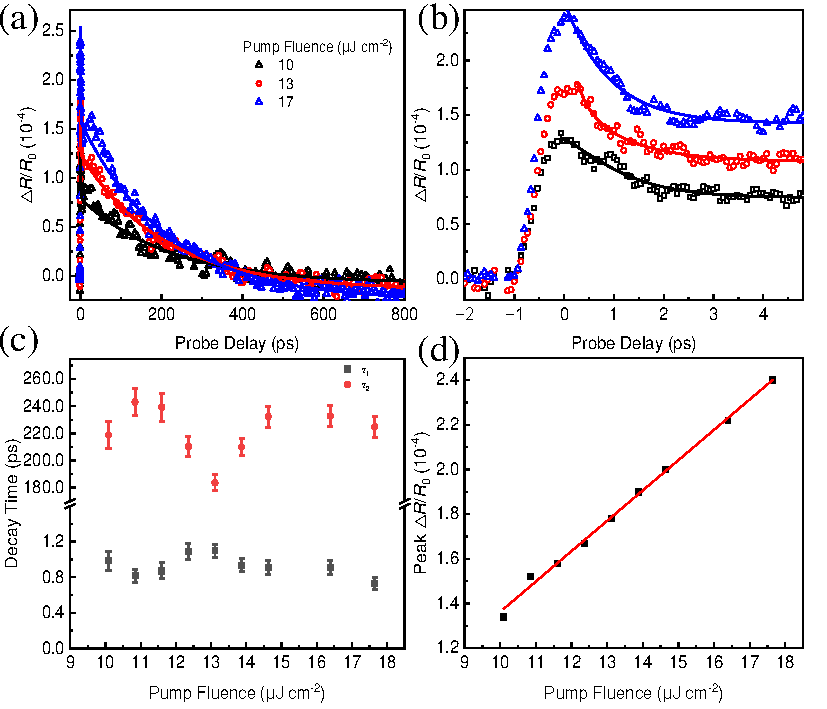
\includegraphics[height=8cm]{example4}
  \caption{(a) Differential reflection signal of the bulk PdSe$_2$ sample as a function of the probe delay measured with an 800 nm probe and a 400 nm pump pulses with various fluences. Curves are exponential fits. (b) The same as (a) but with a shorter range of probe delays. (c) The decay time constants deduced from the fits shown in (b) as a function of the pump fluence. (d) Peak differential reflection signal as a function of the pump fluence. The red line is a linear fit.}
  \label{fgr:example}
\end{figure}

\begin{figure*}[h]
\centering
  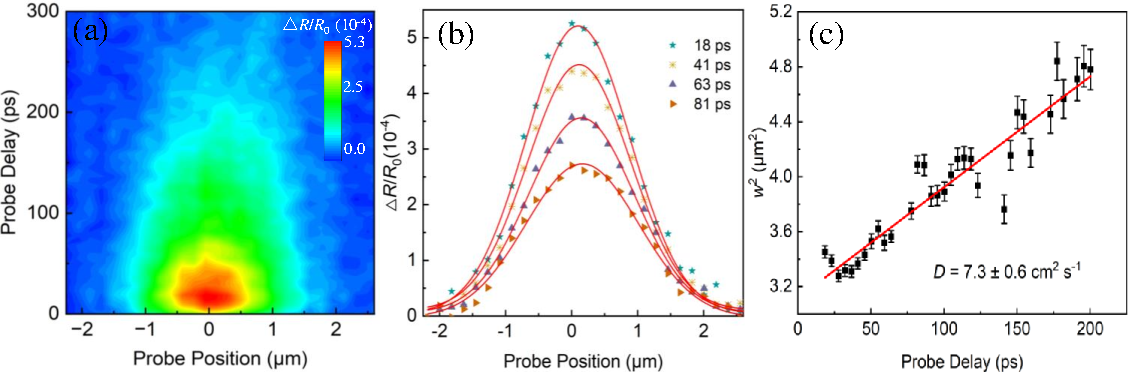
\includegraphics[height=6cm]{example3}
  \caption{(a) Differential reflection signal of the bulk PdSe$_2$ sample as a function of both the probe delay and the probe position. (b) Examples of the spatial profiles of the differential reflection signal at probe delays as labeled in the figure. The red curves are Gaussian fits. (c) The squared width of the spatial profiles obtained by Gaussian fits as a function of the probe delay. The linear fit, shown as the red line, gives a diffusion coefficient of about 7.3 cm$^{2}$ s$^{-1}$. }
  \label{fgr:example}
\end{figure*}

The time-resolved differential reflection measurement of bulk PdSe$_2$ reflects the evolution of the photocarrier density in the sample following their injection by the pump pulse. As depicted in Fig.3a, the signals at various pump fluences exhibit a rapid rise immediately after excitation. Following the peak, the signal decay can be fitted with a double exponential function:

$$ {\Delta}R/R_0  (t)=A_1 \mathrm{exp}(-t/{\tau}_1 )+A_2 \mathrm{exp}(-t/{\tau}_2 )+B,$$
as illustrated by the curves in Fig. 3a. The two decay time constants deduced are plotted in Fig. 3d. We find that these time constants are independent of the pump fluences. The long time constant of approximately 210 ps represents the lifetime of the photocarriers. Notably, this carrier recombination lifetime is longer than that of commonly studied two-dimensional bulk TMDCs, such as WS$_2$  (110 ps),\cite{he2015spatiotemporal} MoTe$_2$ (80 ps),\cite{pan2018understanding} and MoS$_2$ (180 ps).\cite{kumar2013charge}. The short time constant of about 0.87 ps could be attributed to the exciton formation process, as has been generally observed in other TMDCs .\cite{ceballos2016exciton,2017Direct,2018Probing} Fig.3c depicts the relationship between the peak differential reflection signal and the pump fluence. The plot shows that the peak signal is proportional to the pump fluence, further confirming that the differential reflectance is proportional to the carrier density.



To investigate the in-plane transport properties of photocarriers in bulk PdSe$_2$, we conduct a spatially resolved measurement. Fig. 4a illustrates the temporal and spatial evolution of the signal, obtained by scanning the probe delay and position. Driven by the density gradient, the photocarriers are expected to diffuse laterally, resulting in the spatial broadening of the Gaussian distribution over time. Fig.4b presents some examples of the spatial distributions of the differential reflection signal measured at different probe delays of 18 ps (green), 41 ps (yellow), 63 ps (blue), and 81 ps (orange), respectively, along with their Gaussian fits (curves). Fig.4c illustrates the squared Gaussian width as a function of the probe delay. This relation provides insights into the carrier diffusion dynamics and enables the determination of important transport parameters. 



Classical diffusion-recombination model reveals that for photocarriers with an initial Gaussian spatial distribution, the spatial profile maintains a Gaussian shape throughout the diffusion and recombination process. The full-width at half-maxima of the spatial profile evolves as
$$ w^2(t)=w_0^2+16\mathrm{ln} (2) Dt$$
here, $D$ and $w_0$ denote the carrier diffusion coefficient and the initial Gaussian profile width.\cite{Ceballos2017Ultrafast} The red line in Fig. 4c represents a linear fit, from which we extract a diffusion coefficient of 7.3 cm$^{2}$ s$^{-1}$. Multiple measurements were performed on this sample, and similar results have been obtained as shown in Fig. S1 and Fig. S2, Supporting Information.

Using the lifetime (210 ps) obtained above, the diffusion length ($L$) in bulk PdSe$_2$ can be calculated as 400 nm. Furthermore, by applying the Einstein relation, a photocarrier mobility of approximately 300 cm$^{2}$ V$^{-1}$ s$^{-1}$ can be obtained. This mobility value is comparable to those reported in the literature $^{14}$ and highlights the advancements in optoelectronic device fabrication technology. It is worth noting that the diffusion coefficient and diffusion length measured in our experiment are larger than the previously reported values of typical TMDC crystals. For instance, the diffusion coefficient and length bulk WS$_2$ is 3.5 cm$^{2}$ s$^{-1}$ and 196 nm, respectively,\cite{he2015spatiotemporal} and 4.2 cm$^{2}$ s$^{-1}$ and 270 nm, respectively, in bulk MoS$_2$.\cite{kumar2013charge}








Other basic parameters of carrier dynamics can be extracted from these results. The observed diffusion of carriers is driven by density gradients through thermal motion of the carriers. At room temperature, the thermal velocity of the carriers is approximately 10$^{5}$ m/s. With a diffusion coefficient of 7.3 cm$^{2}$ s$^{-1}$, the corresponding mean free time is 0.073 ps, and the mean free path is 7.3 nm. The insights gained into carrier dynamics and transport properties provide a theoretical basis for the development of new microdevices based on PdSe$_2$ in the fields of optoelectronics and electronics.

\section{Conclusions}
This study provides insights into the dynamical behavior of photocarriers in bulk PdSe$_2$ using spatiotemporally resolved transient absorption microscopy. We obtain a recombination lifetime of approximately 210 ps, a photocarrier diffusion coefficient of approximately 7.3 cm$^{2}$ s$^{-1}$, a diffusion length of about 400 nm, and a mobility of around 300 cm$^{2}$ V$^{-1}$ s$^{-1}$. These findings enhance our understanding of optoelectronic properties of PdSe$_2$. This knowledge serves as a solid foundation for future material advancements and provides a basis for designing optoelectronic devices with optimal performance using this novel material.


\section*{Conflicts of interest}
The authors declare no conflict of interest.

\section*{Acknowledgements}
We are grateful for the financial support of the National Natural Science Foundation of China (Grant No. 61975007) and the Beijing Natural Science Foundation (Grant Nos. Z190006 and 4222073). H.Z. acknowledges support by the U.S. Department of Energy (DE-SC0020995). 

%%%END OF MAIN TEXT%%%

%The \balance command can be used to balance the columns on the final page if desired. It should be placed anywhere within the first column of the last page.

\balance

%If notes are included in your references you can change the title from 'References' to 'Notes and references' using the following command:
%\renewcommand\refname{Notes and references}

%%%REFERENCES%%%
\bibliography{rsc} %You need to replace "rsc" on this line with the name of your .bib file
\bibliographystyle{rsc} %the RSC's .bst file


\end{document}
